\documentclass[multi,preview,varwidth=false,border=5,12pt]{standalone}
%\documentclass[12pt]{article}

\newcounter{Qnum}
\usepackage{assignments}
\standaloneenv{question}


\excludecomment{solution}\let\endsolution\relax


\begin{document}

\begin{center}
\section*{General Energy Equation}
\end{center}

\begin{question}

A horizontal pipe carries oil with a specific gravity of 0.86.  Two pressure gauges placed along the pipe read 80 psig and 60 psig.  What is the energy loss (in feet) between the two gauges.

\begin{solution}
\end{solution}

\end{question}


\begin{question}

Turpentine is flowing at $0.45~\m^3/s$ in the fabricated tube shown below.  There is an energy loss of 0.7 $\N\cdot \m/\N$ as the Turpentine travels through the gradual enlargement.  If the pressure before the enlargement at A is 500 kPa what is the pressure at point B?

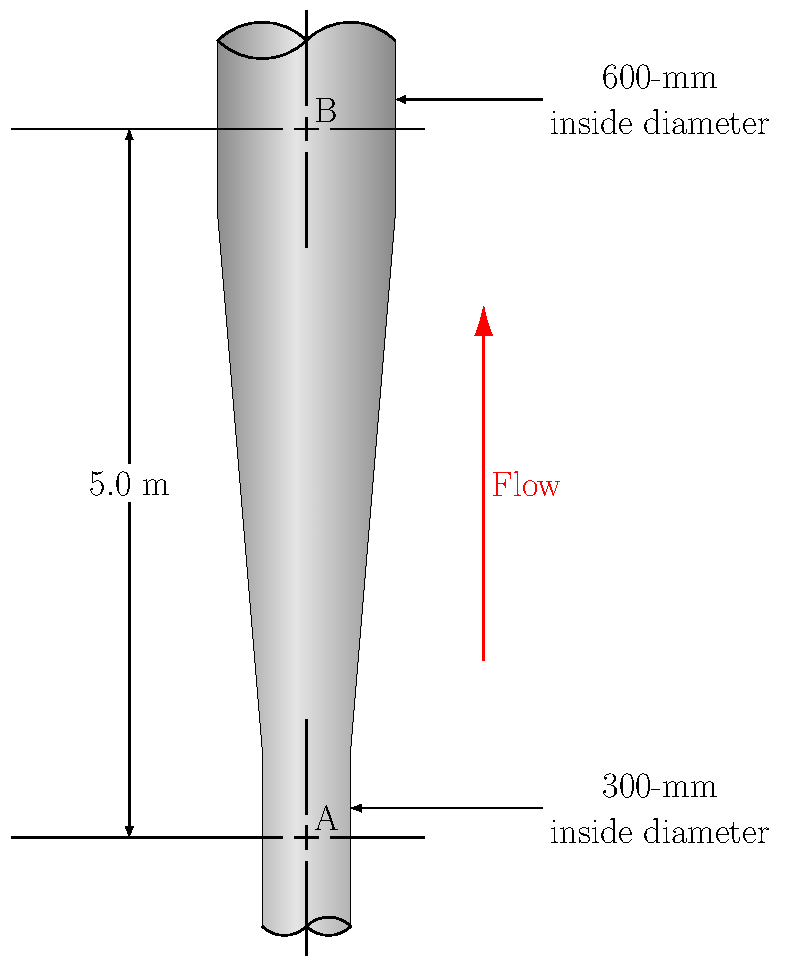
\includegraphics[width=3in]{imgs/PipeExp1.pdf}

\begin{solution}

First note that the value of $h_L=0.7$ is ten times larger than I expect for the gradual enlargement that occurs over 5 meters ($K\approx 0.035$).  This is closer to the loss expected for a sudden enlargement ($K\approx 0.5$).

$$
\frac{p_A}{\gamma}+z_A+\frac{v_A^2}{2g}-h_L=\frac{p_B}{\gamma}+z_B+\frac{v_B^2}{2g}
$$

Note that flow is from $A \to B$.


\begin{align*}
p_A &= 500~\kPa \\
\gamma &=8.53~\kN/\m^3 \\
z_A &=0 \\
z_B &= 5~\m \\
v_A &=\frac{Q}{A}=6.366~\m/s \\
v_B &=1.592~\m/s
\end{align*}

$$
p_B=p_A+\gamma\left(z_A-z_B\right)+\frac{\gamma}{2g}\left(v_A^2-v_B^2\right)-\gamma h_L
$$

$$
p_B=500~\kPa-42.65~\kPa+16.52~\kPa-5.97~\kPa
$$

$$
p_B=473.87~\kPa-5.97~\kPa=467.9~\kPa
$$

\end{solution}

\end{question}



\begin{question}

Water flows from the large tank at a rate of 1.1 ft$^3$/s through the pipe system shown below.  The piping is 4-in schedule 40 steel.  How much energy is lost from the system?  Report your answer as a head in feet.

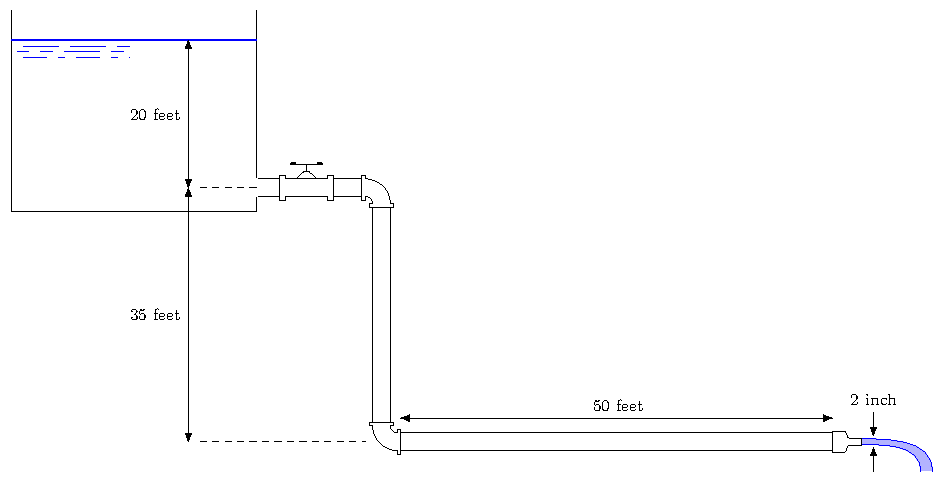
\includegraphics[width=5in]{imgs/TankGateElbows.pdf}


\begin{solution}
15.5 feet
\end{solution}

\end{question}


\begin{question}

A manufacturer of a centrifugal pump reports that 30 hp is required to pump 1000 gpm of water at a head of 80 ft.  What is the efficiency (in percent) of this pump under these operating conditions?

\end{question}


\begin{question}

A pump is used to transfer water from an open tank to a closed tank containing air at 500 kPa above the water.  If the pump has an efficiency of 80\%, how much power is consumed when transferring 2000 L/min of water?  Assume that the water level in both tanks are the same.

What would be the power consumed if the tank on the left was sealed with an air pressure of 100 kPa?

Report your answers in kW.

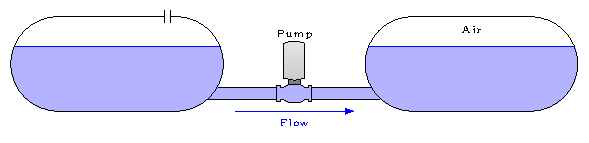
\includegraphics[width=5in]{imgs/PumpTransfer.pdf}


\end{question}


\end{document}
